\chapter{Analyse der Informationsquellen in eines Unternehmensnetzwerkes}
\label{cha:Analyse der Informationsquellen in eines Unternehmensnetzwerkes}

SIEM Systeme sind, vor allem in großen Unternehmensnetzwerken (siehe SANS Paper Proactive)
\todoForm{Unternehmensanalyse: Quelle einfügen für Aussage bzgl. SIEM Einsatz (SANS Paper Proactive)!}
, zu einem Standard geworden, um Informationen aus Protokollen verschiedener Systeme und anderen Kontextdaten zu gewinnen und diese in Szenarios einzuordnen. Um das Zwischenziel einer Bewertung der aktuellen Informationsmenge eines industriellen Netzwerkes zu erhalten, bietet es sich durch diesen Zustand an, einen Abgleich zwischen dem, in Bezug auf SIEM Technologie, etablierten Informationstand in Unternehmensnetzwerken und industriellen Netzwerken auszuführen. In diesem Kapitel soll es deshalb um eine akkurate Beschreibung der Informationsmenge eines typischen Unternehmensnetzwerkes gehen, die aus einer Analyse der gängigen Informationstypen und -kategorien erfolgt. Dazu wird im folgenden zunächst der Analyseansatz geschildert, der das Vorgehen schildert und die Analyse nachvollziehbar gestalten soll.

\section{Verwendete Analysemethode}

% Schritt 1: Recherchiere welche Log Dateien existieren
% Schritt 2: Jede Log Datei auf einem System ansehen und Eventformate heraussuchen
% Schritt 3: Events nach Typ kategorisieren
% Schritt 4: 

%Ziel der Analyse
Die erste Frage für die Wahl des Analyseansatzes stellt sich sowohl in der gewählten Tiefe als auch in einer zielgerichteten Methodik. Das Ziel der Analyse liegt darin, die sicherheitsrelevante Infortmationsmenge zu erfassen. Informationen werden als sicherheitsrelevant betrachtet, wenn diese Informationen genutzt werden können, um die Nutzung eines bestimmten Angriffsvektors erkennen zu können. Da Angriffsvektoren und die möglichen Folgeschritte sehr zahlreich und spezifisch für ein bestimmtes System oder eine Applikation sein können, ist eine allumfassende Analyse aller Angriffsvektoren nicht möglich. Deshalb wird in dieser Analyse von einem vereinfachten Modell ausgegangen, um eine Einschätzung der möglichen Informationsmenge zu erhalten. 

\begin{figure}[h]
\centering
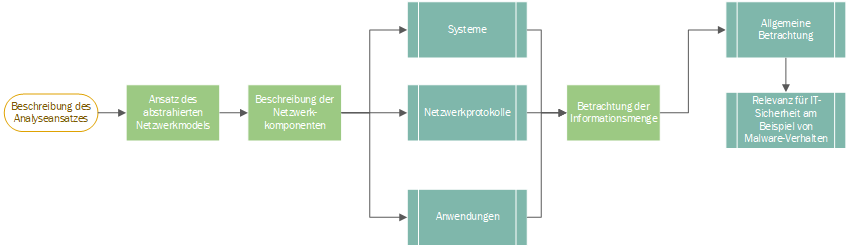
\includegraphics[width=125mm]{Zeichnungen/Analyseansatz.png}
\caption{Analysestruktur (Placeholder)}
\label{fig:Analysestruktur (Placeholder)}
\end{figure}

%Beschreibung der eigenen Durchführung
Basierend auf diesen Praktiken ergibt sich die Durchführung der Analyse: Zunächst werden das benutzte Modell und dessen Komponenten beschrieben. Das Ziel der Beschreibung der Komponenten ist es, einen Überblick über die verfügbaren Informationsquellen zu definieren. Darauf folgend wird auf Basis der Informationsmenge eine Einteilung der Informationen in Kategorien vorgenommen, die eine Basis für den Vergleich der Informationsmengen bilden.
Um die Auswahl der Kategorien zu verdeutlichen, wird desweiteren anhand des Beispiels einer Malware-Analyse aufgezeigt, welche Indikatoren auf das Eindringen einer Malware in den verschiedenen Schritten hinweisen können.


\section{Beschreibung des Modells}

%Kommentar: Vielleicht macht es Sinn erst die Elemente und dann die Architektur zu beschreiben...

%Ziel 1: Beschreibung der ausgewählten Kernfaktoren basierend auf der Grundlagenrecherche
%Ziel 2: Beschreibung der Architektur & Interaktionen als Grundlage der Analyse

%Architekturidee:
%Router <--> Firewall <--> DMZ (Webserver mit Webservice) <--> Firewall <--> Intranet (User PC) <--> Firewall <--> Restricted Zone (Database Server & SIEM)

Das Ziel des Modells ist es eine repräsentative, vereinfachte Darstellung eines Unternehmensnetzwerkes mit typischen Komponenten für den Betrieb darzustellen. Der Aufbau des Netzwerkes orientiert sich an typischen Elementen, die in einem Unternehmensnetzwerk zu finden sind. Dabei besteht die Notwendigkeit, das Modell in seiner Größe und Komplexität einzugrenzen, um eine Analyse in sinnvollem Maße zu ermöglichen, gleichzeitig aber ein möglichst vollständiges Bild erhalten zu können.

Die Architektur und Einteilung in verschiedene Netzwerkzonen ist dabei von üblichen Sicherheitszonen abgeleitet. Während die Positionierung der Elemente keine besondere Rolle spielt in Bezug auf die ermittelbaren Informationen pro Element, ist jedoch anzumerken, dass auch diese Informationen, z.B. in Form der Auswertung von Netzwerkadressen, einem SIEM-System nützliche Informationen zur Verfügung stellen können. Aus diesem Grund werden die Zonen beispielhaft in das Modell integriert. Die Architektur des Modells beginnt an seinem \glqq Rand\grqq , dem Zugang zum WAN (Internet), über einen Gateway-Router. Dieser Router ermöglicht die Weiterleitung von Netzwerkpaketen in und aus der angrenzenden Netzwerkzone, der de-militarisierten Zone (DMZ). 
%In der DMZ sind für dieses Modell jeweils ein Apache Webserver 
In der DMZ des Modells ist ein Apache Webserver auf der Basis des Betriebssystems \glqq CentOS (Linux)\grqq{} platziert. Dieses Element bietet die Möglichkeit, Datenverkehr über das Hypertext Transport Protocol (HTTP) sowie die verfügbaren Protokolleinträge eines Webservers und eines Linux-basierten Servers zu untersuchen. Alle Elemente werden durch \glqq Managed Switches\grqq{}  miteinander verbunden.

Die DMZ wird von der nächsten Zone, dem Extranet, durch eine Firewall überwacht, die eingehende initiale Kommunikation blockiert. Firewalls gehören zu den Grundlagen der Sicherheit von Unternehmen und werden häufig platziert, um Datenverkehr in und aus bestimmten Netzwerkzonen zu überwachen. Innerhalb der Netzwerkzone werden zwei Benutzer-PCs eingesetzt. Diese werden platziert, um Abweichungen und andere Benutzerinteraktionen in die erhaltbare Informationsmenge zu integrieren. Die beiden Computer unterscheiden sich wie auch die Server der DMZ im Betriebssystem, sodass ein PC auf Basis des Windows-Betriebssystem enthalten ist.

Als dritte Netzwerkzone wird als \glqq Restricted Area\grqq{}  bezeichnet. Innerhalb dieser Netzwerkzone wird ein Windows-basierter Server eingesetzt. Auf diesem Server wird ein Microsoft SQL Datenbankserver ausgeführt, um kritische Unternehmensdaten abzubilden. Diese Elemente ermöglichen die Untersuchung eines Windows-basierten Betriebssystems sowie die Verwendung eines Datenbankservers und der dazugehörigen Protokoll-Suite.
Zusätzlich ist in dieser Zone als Ergänzung auch der SIEM-Server gesetzt.

Zwischen den verschiedenen Elementen des Netzwerkes werden Informationen ausgetauscht, z.B. für die Abfrage einer Ressource, Herstellung einer Kommunikation oder Übermittlung von Authentifizierungsinformationen. Dieser Austausch wird durch verschiedene Protokolle gesteuert. Der Inhalt der gesendeten Datenpakete (Payload) wird mit verschiedenen Header-Informationen gekapselt. Neben den grundlegenden Header-Daten der Protokolle auf niedrigeren Ebenen (Ethernet, IP, TCP/UDP) sollen in diesem auch verschiedene Protokolle der Ebene 7 betrachtet werden. Die zugehörigen Header-Information sind spezifisch für das entsprechende Protokoll und können z.B. Informationen über den Status der Kommunikation beinhalten. Diese Informationen sind bei der Analyse von Netzwerkdaten nützlich, um den Kontext der ausgetauschten Daten zu verstehen und einen Ablauf der Kommunikation nachzuvollziehen.
In dem verwendeten Modell werden verschiedene Protokolle bei der Kommunikation zwischen den verschiedenen Komponenten betrachtet. Die Wahl des Protokolls hängt von der spezifischen Schnittstelle ab. Eine Auflistung der Schnittstellen für das Ansprechen der entsprechenden Komponente werden in der folgenden Tabelle aufgelistet:

Kommunikationsschnittstellen:
\begin{itemize}
\item Microsoft SQL Datenbank: SQL Protocol Suite
\item Fernzugriff auf ein System: SSH, RDP
\item WebServer: HTTP
\end{itemize}

Die Betrachtung der Informationen von den Netzwerkelementen und der Kommunikation zwischen den Elementen ergibt das Gesamtbild der ermittelbaren Informationsmenge in diesem Modell. Die folgenden Schritte betrachten beide Teile für die jeweils zu untersuchenden Elemente.

\section{Beschreibung der Systeme}
\subsection{Windows}
Das Windows Betriebssystem von Microsoft ist das am Weitesten verbreitete Betriebssystem in der Industrie. Wollen wir die Informationsmenge eines Windowssystemes beschreiben, können wir auf verschiedene Punkte zurückgreifen. In Bezug auf Angriffsanalysen und forensische Analyseverfahren werden zu diesem Zweck drei grundlegende Teile betrachtet: Protokolldateien des Betriebssystems sowie installierter Software, die Windows Registry und ausgeführte Prozesse. Die Überwachung und Dokumentation dieser Bereiche ermöglicht, es ein Bild über den aktuellen Zustand des Systems zu erhalten. 
Für die Ausführung von Prozessen und Änderungen der Registry kann eine installierte Überwachungssoftware in Form einer lokalen, systemfokussierten Lösung genutzt werden. Mit Hilfe einer solchen Lösung ist es möglich, die Ausführung von Dateien oder das Laden dynamischer Bibliotheken zu überwachen und Sicherheitsereignisse,  im Falle der Ausführung/des Ladens aus ungewöhnlichen oder für diesen Zweck gesperrten Verzeichnissen des Dateisystems, zu generieren. Selbiges gilt für Änderungen von Schlüsseln innerhalb der Registry. 

Der dritte Teil besteht aus den Protokolldateien des Betriebssystems. 

%Beschreibung der grundlegenden Logdateien
%Quelle: https://technet.microsoft.com/de-de/library/cc722404(v=ws.11).aspx
Das Windowsbetriebssystem beinhaltet zwei Kategorien für Protokolldateien: Windows Protokolle und Dienst- und Anwendungsprotokolle. 
Die Windowsprotokolle beinhalten Ereignisse, die durch das Betriebssystem protokolliert werden. Diese werden einer von fünf Protokolldateien zugeordnet: \textit{Anwendung}, \textit{Sicherheit}, \textit{Installation}, \textit{System} und \textit{Weitergeleitete Ereignisse}. \\

Das Anwendungsprotokoll beinhaltet Ereignisse, die von installierten Anwendungen protokolliert werden und etwa Fehler mit Bezug auf das Dateisystem signalisieren. Welche Ereignisse konkret protokolliert werden, wird von den Entwicklern der Anwendung bestimmt. 

Das Sicherheitsprotokoll beinhaltet Ereignisse bzgl. sicherheitsrelevanter Elemente wie z.B. Fehlern bei der Anmeldung eines Benutzers oder bzgl. der Ressourcenverwendung bei der Erstellung, Öffnung und Löschung von Objekten. Die Administratoren des Betriebssystems entscheiden, welche Ereignisse dieser Kategorie protokolliert werden. 

Das Systemprotokoll enthält Ereignisse, die von Systemkomponenten des Betriebssystems protokolliert werden, während das Setupprotokoll Ereignisse sichert, die bei der Installation von Anwendungen auftreten können \citep{MS2}.\\

Die zweite Kategorie, Anwendungs- und Dienstprotokolle, beinhaltet Protokolle, deren Ereignisse im Kontext von einzelnen Programmen auftreten und keine systemweiten Auswirkungen haben. Diese Kategorie wird in vier Unterkategorien unterteilt: \textit{Verwaltung}, \textit{Betrieb}, \textit{Analyse} und \textit{Debug}. 


Verwaltungsprotokolle enthalten Ereignisse mit Problemen und vordefinierten Lösungspfaden für Administratoren. 

Betriebsprotokolle enthalten Ereignisse, deren Daten für die Analyse und Diagnose von auftretenden Problemen sowie für das Auslösen von installierten Werkzeugen oder Programmen genutzt werden können. 

Die Analyse- und Debugprotokolle sind standardmäßig deaktiviert und müssen für die Verwendung aktiviert werden. Dabei enthält das Analyseprotokoll Ereignisse zu Programmoperationen und Problemen, die nicht vom Benutzer behoben werden können, während das Debugprotokoll weitere Daten für Entwickler beinhaltet. \\

%Beschreibung des Aufbaus der Logdateien
Die Protokolldateien sind in einem spezifischen Format geschrieben, sodass eine Anzahl an Feldern vorgegeben ist, die durch den bereitstellenden Service bzw. den bereitstellenden Prozess gefüllt werden können. Die Protokolldateien werden im EVT (alt) bzw. EVTX (neu) Format dargestellt. In der, vom Betriebssystem bereitgestellten, Ereignisanzeige können die Daten sowohl in benutzerfreundlicher Formatierung als auch in einer XML-basierten Form dargestellt werden. Die folgenden Felder werden für diese Protokolle bereitgestellt:
\begin{itemize}
\item Quelle
\item Ereignis-ID
\item Ebene
\item Benutzer
\item Vorgangscode
\item Protokoll
\item Aufgabenkategorie
\item Schlüsselwörter
\item Computer
\item Datum und Uhrzeit
\item Zusätzliche Felder: Prozess-ID, Thread-ID, Prozessor-ID, Sitzungs-ID, Kernelzeit, Benutzerzeit, Prozessorzeit, Korrelations-ID und relative Korrelations-ID
\end{itemize}
\todoImage{Bild für Windowslog Eventfelder einfügen zur Verdeutlichung}
%Quelle: https://technet.microsoft.com/de-de/library/cc765981(v=ws.11).aspx
Diese Felder können durch die jeweilige Quelle und das Betriebssystem mit verfügbaren Daten versehen werden.\\ 

Die Quelle gibt die Software(-komponente) oder die Komponente des Betriebssystems an, die das Ereignis protokolliert hat. Die zugehörige Ereignis-ID benennt den Ereignistypen, der z.B. das erfolgreiche Starten eines spezifischen Dienstes darstellt. Weitere Identifikatoren geben spezifischere Informationen über den auslösenden Prozess und zugehörige Elemente an.


Jedes Ereignis wird zu einer bestimmten Kategorie zugeordnet, der Ebene. Die Ebene eines Ereignisses bezeichnet den zugeordneten Schweregrad des Ereignisses. Für alle Protokolldateien stehen die folgenden Ebenen zur Verfügung: \textit{Informationen}, \textit{Warnung}, \textit{Fehler} und \textit{Kritisch}. \\


Ereignisse der Ebene \textit{Informationen} enthalten Daten über Änderungen an Anwendungen oder Komponenten. Der erfolgreiche Start bzw. die erfolgreiche Beendigung eines Dienstes, sofern dieser nicht die Systemfunktionalität o.ä. gefährdet, seien hier als Beispiel genannt. 

Die Ebenen \textit{Warnung} und \textit{Fehler} weisen auf Ereignisse hin, die das Auftreten eines Problems signalisieren.
Die Ebene \textit{Warnung} beschreibt Ereignisse, die das Auftreten eines Problems anzeigen, durch das ggf. ein Fehler ausgelöst oder ein Dienst beeinträchtigt werden könnte. Ein Beispiel ist die Verzögerung der Ausführung des Herunterfahrens des Betriebssystems durch einen Prozess, dessen Beendigung verzögert oder nicht durchgeführt werden kann. Die Ebene \textit{Fehler} beschreibt Ereignisse, die potentiell die Funktionalität außerhalb der protokollierenden Quelle beeinträchtigen können. Die Bewertung der Ereignisse dieser Ebene sind somit als schwerwiegender anzusehen als Ereignisse der Ebene Warnung.


Die letzte Ebene \textit{Kritisch} umfasst Ereignisse, die Fehler signalisieren, jedoch nicht automatisch von dem Betriebssystem behoben werden können. 

In Protokolldatei \textit{Sicherheit} treten dazu noch zwei weitere Ebenen auf: \glqq Erfolgsüberwachung\grqq{} und \glqq Fehlerüberwachung\grqq . Diese Ebenen umfassen Ereignisse, die mit der Anwendung der Rechte des ausführenden Benutzers zusammenhängen. Ereignisse der Ebene Erfolgsüberwachung beinhalten die Dokumentation der erfolgreichen Anwendung der Rechte, Ereignisse der Ebene Fehlerüberwachung beinhalten Fehlermeldungen, die bei der Anwendung aufgetreten sind \citep{MS1}.

%Quelle: https://support.microsoft.com/en-us/help/942910/-error--warning--or-critical-events-are-logged-in-the-diagnostic-perfo
Ereignisse der gleichen Quelle und der gleichen Event-ID können abhängig vom Schweregrad in den verschiedenen Ebenen eingeordnet werden.\\


%Beschreibung der Sicherheitslogdatei im Detail
%Quelle: https://support.microsoft.com/en-us/help/977519/description-of-security-events-in-windows-7-and-in-windows-server-2008
In der Protokolldatei \glqq Sicherheit\grqq{} konnten bei einer Untersuchung eines in der Produktion eingesetzten Windowsservers die mit Abstand größte Zahl an Ereignissen festgestellt werden. Im Sicherheitsprotokoll werden Ereignisse festgehalten, die verschiedene Komponenten bzgl. der Sicherung des lokalen Servers oder Computers als auch Zugriffe auf geteilte Resourcen innerhalb einer Windowsdomäne oder mehrere Domänen betreffen. Im Detail können diese Kategorien einen guten Einblick über die Merkmale der überwachten Elemente durch das Betriebssystems geben:
\begin{itemize}
\item Account Logon
\item Account Management
\item Detailed Tracking
\item DS (Directory Service) Access
\item Logon/Logoff
\item Object Access
\item Policy Change
\item Privilege Use
\item System
\end{itemize}
%Beschreibe jede Kategorie
Grundsätzlich lassen sich die Unterkategorien bzw. Ereignisse in zwei Bereiche unterteilen: \textit{Domänen- bzw. Directory Service basierte} Ereignisse und \textit{lokale} Ereignisse. Erstere Ereignistypen beziehen sich auf den Zugang zu Domänen und allgemeine Zugriffs- und Rechteverwaltung sowie auf die technisch darunterliegenden Protokolle und Services. Lokale Ereignistypen beziehen sich auf lokale Ereignisse bzgl. des Zugangs zu dem Betriebsystem und die Benutzung von Privilegien und die damit verbundenen Sicherheitsrichtlinien\citep{MS3}. \\

%DS
Zu den Kategorien der Directory Services zählen \textit{Account Logon}, \textit{Account Management} und \textit{DS Access}.

Die Kategorie \glqq Account Logon\grqq{} bezeichnet nicht die Authentisierung eines Benutzers an einem Windowsbetriebssystem, sondern die Funktionalität des Kerberosservices. Kerberos ist ein verteilter Authentifizierungsdienst, der für die Anmeldung an einer Windowsdomäne verwendet wird.  Daher beziehen sich Ereignisse aus dieser Kategorie auf Operationen bzw. Eigenschaften des Kerberosprotokolls. 

Die verwandte Kategorie \glqq Account Management\grqq{}  bezieht sich auf die Verwaltung von Distribution Groups (Verteilungsgruppen für E-Mail Services) und Security Groups (Zuordnung von Benutzerrechten und Zugriffsrechten auf geteilte Resourcen). Desweiteren enthält diese Kategorie auch Informationen zu der Erstellung von Accounts sowie Zugriffsversuchen auf Passworthashs und Anfragen an die Passwortrichtlinienschnittstelle. 

Eine technische Kategorie des Verzeichnisdienstes wird durch \glqq DS Access\grqq{}  gebildet. Diese Kategorie enthält Ereignisse bzgl. Änderungen, Zugriffen und Replikationen des Verzeichnisdienstes bzw. der im Verzeichnisdienst enthaltenen Daten \citep{MS3}. \\

%Lokal
Die Kategorien des lokalen Ereignisbereiches sind \textit{Detailed Tracking}, \textit{Logon/Logoff}, \textit{Object Access}, \textit{Policy Change}, \textit{Privilege Use} und \textit{System}.

\glqq Detailed Tracking\grqq{}  weißt auf Ereignisse bzgl. der Erstellung und Vernichtung von Prozessen hin sowie Aktiviten bzgl. der Data Protection Schnittstelle \glqq DPAPI\grqq{}  und Anfragen auf die RPC (Remote Procedure Call)-Schnittstelle.

Die Kategorie \glqq Logon/Logoff\grqq{} kann als äquivalente lokale Kategorie gesehen werden, da diese Ereignisse bzgl. der Anmeldung/Abmeldung als lokaler Benutzer an einem Betriebssystem gesehen werden kann. Allerdings enthält diese Kategorie auch Ereignisse bzgl. der Nutzung des IPSec Protokolls und die Interaktion eines Benutzers mit einem Network Policy Server. 

Die Kategorie \glqq Object Access\grqq{} stellt Ereignisse bzgl. des Zugriffes und der Änderung auf systemrelevante Objekte dar. So sind Ereignisse bzgl. der Verbindung zur Windows Filtering Plattform, darunter Ereignisse der Windows Firewall. Die Windows Filtering Platform ist eine Sammlung aus Schnittstellen und Systemdiensten, die für die Erstellung von Programmen zur FIlterung und Modifikation von Netzwerkdatenverkehr genutzt werden kann. Die Windows Firewall basiert auf dieser Sammlung \citep{MS4}. 
%Quelle: https://msdn.microsoft.com/de-de/library/windows/desktop/aa366510(v=vs.85).aspx
Desweiteren werden dieser Kategorie Ereignisse zugeordnet bzgl. Änderungen der Windows Registry Keys, des Component Object Models (COM+), Zugriffe auf das Dateisystem und geteilte Verzeichnisse sowie die Manipulation von Zugriffsoptionen auf Systemressourcen und Änderungen am Certification Service \citep{MS3}. 

Die Kategorie \glqq Policy Change\grqq{} beschreibt Ereignisse, die mit der Änderungen von Richtlinien-Objekten zusammenhängen. Die entsprechenden Richtlinien gehören zu den Bereichen Authentisierung, Authorisierung, Überwachung, Windows Filtering Platform sowie des MPSSVC (Teil der Windows Firewall, welcher vor nicht-autorisiertem Zugriff von Benutzern aus dem Internet oder einem Netzwerk schützt) und anderer Richtlinien (z.B. in Bezug auf kryptografische Operationen) \citep{MS5}. %Quelle: https://technet.microsoft.com/de-de/library/cc722146(v=ws.10).aspx

Die Kategorie \glqq Privilege Use\grqq{}  beinhaltet Ereignisse zu der (nicht-)sensiblen Benutzung von Privilegien im Kontext des Betriebssystems \citep{MS3}. 
Schlussendlich zeigen Ereignisse aus der Kategorie \glqq System\grqq{}  Änderungen am (Sicherheits-)Zustand des Systems sowie der Sicherheitssubsysteme (Local Security Authority und Security Account Manager) \citep{MS3}. \\

%Kategorisierung der Quellen der Beispiellogs von produktiven Servern
Ereignisse der genannten Quellen können auch, abhängig von der ID, also dem Ereignistypen, in anderen Protokollen wie etwa dem Anwendungsprotokoll oder dem Systemprotokoll aufgeführt werden.
\todoForm{Windows Protokolle: Ggf. weitere Beispiele nennen, kurz beschreiben}

%Beispiele für andere Anwendungen
Neben den fundamentalen Protokolldateien können weitere Protokolldateien von Applikation erstellt werden. Neben Microsoft-Produkten wie dem Webserver IIS, Microsoft Office oder der Benutzerverwaltung Active Directory können auch Protokolle von Microsoft-fernen Produkten wie z.B. einer Anti-Virensoftware oder proprietäre Netzwerkdienste durch die Applikationen zur Verfügung gestellt werden.
\todoQuestion{Loggt das Betriebssystem Elemente aus diesem Bereich? Wie funktioniert die Anbindung der Protokolldateien an das Betriebssystem?}
%Frage: Warum lasse ich Elemente wie z.B. eine zentrale Benutzerverwaltung raus? Ist das nicht eigentlich relevant?
%Antwort: Die zentrale Frage hier ist: Welche Daten bekomme ich, in Bezug auf den normalen PC, aus einer Benutzerverwaltung wie z.B. einem Active Directory, die ich nicht aus einem Windowssystem bekomme?
%Um diese Frage zu beantworten müsste ich wissen nach welchen Informationen ich suche im Bezug auf die Benutzerverwaltung?
%Brainstorming: Login/Logoff von Benutzern (beide), Berechtigungen des Benutzers (beide), Zertifizierung? (nur AD), 
%Zentrale Frage des IAMs: Wer (Login) hat was (Lokale Prozessevents, Netzwerkdaten) wann (Timestamps, generell) wo (Kombination der Elemente) wie (Kombination der Elemente) gemacht?
%Spezifizierte Frage: Welche Kontextinformationen bekomme ich von einer zentralen Benutzerverwaltung, die ich nicht von einem lokalen System bekomme?
%Ansatz: Erstmal Windows anschauen, dann ggf. nach AD suchen
%Temporäres Resultat: AD erstmal weglassen, später einbauen

\subsection{Linux}
Für die Extraktion der Informationsmenge aus einem Linuxsystem wird die gleiche analytische Basis wie für das Windowsbetriebssystem vorausgesetzt. Die Betriebssysteme unterscheiden sich von ihrem Aufbau und ihren Mechanismen teilweise deutlich, jedoch lässt sich der Grundsatz ähnlich ableiten. Das Ziel ist es, alle verfügbaren Informationen zu erhalten, die bei der Ausführung des Systems entstehen. Dies schließt die Analyse von Protokollen ein sowie die Überwachung der Ausführung von Diensten (Services) und die Ausführung von (System-)Prozessen. \\

In Bezug auf das Betriebssystem Linux sollen daher die vorhandenen Protokolle sowie grundlegende Elemente, wie etwa zugehörige Informationen zu Diensten und Informationen über die Ausführung von Befehlen, untersucht werden.

%Logfiles
Bei Linux unterscheidet man zwischen verschiedenen Distributionen. In Bezug auf Protokolldateien differenziert man in der Literatur bzgl. der Namensgebung zwischen Debian-basierten Distributionen wie etwa Ubuntu und CentOS/RedHat. 
%Quelle https://www.eurovps.com/blog/important-linux-log-files-you-must-be-monitoring/
In Linux existieren vier typische Kategorien für Protokolldateien \citep{Linux1}:
\begin{itemize}
\item Application Logs
\item Event Logs
\item Service Logs
\item System Logs
\end{itemize}


%Syslogd
%Quelle1: https://www.thegeekdiary.com/centos-redhat-beginners-guide-to-log-file-administration/
%Quelle2: http://www.linux-community.de/Community/Fragen/HOWTO-linux-logfiles
Unter Linux wird das Protokollieren von Systemmeldungen durch \glqq syslogd\grqq{}  übernommen, den \glqq system logging daemon\grqq . Desweiteren protokolliert der Daemon \glqq klogd\grqq{} Ereignismeldungen aus dem Kernel (Betriebssystemkern). Diese beiden Prozesse, die im Hintergrund ausgeführt werden, schreiben Meldungen in Protokolldateien, die sich in dem Unterverzeichnis \glqq syslog\grqq{}  (Debian-basiert / Ubuntu) bzw. \glqq messages\grqq{}  (CentOS / RedHat) des Standardverzeichnis für Protokolldateien befinden (/var/log/). Dabei werden die Meldungen als Ereignisse durch Regeln den verschiedenen Protokolldateien zugeordnet, abhängig von ihrer \glqq Facility\grqq{}  sowie ihrer Priorität. 

Für rsyslogd bestehen die folgenden Facilities:
\begin{itemize}
\item auth/authpriv: Security/authorization messages (private)
\item cron: Clock daemon (crond \& atd)
\item Daemon Messages from system daemons
\item kern: Kernel messages
\item local0-local7: Reserved for local use
\item lpr: line printer subsystem
\item mail: Messages from mail daemons
\item news: USENET news subsystem
\item syslog: Messages generated internally by system log daemon
\item User: Generic user-level messages
\item UUCP: UUCP subsystem
\end{itemize}

Für jedes Ereignis werden, ähnlich der Ebene für Windowsprotokolle, Prioritäten vergeben:
\begin{itemize}
\item emerg: System is unusable
\item Alert: Action must be taken immediately
\item crit: critical conditions
\item err: error conditions
\item warning: Warning conditions
\item notice: normal but significant importance
\item info: informational messages
\item debug: debugging messages
\end{itemize}

Basierend auf diesen Parametern werden die Ereignisse in die Protokolldateien geschrieben, deren Namen auf diesen Parametern basieren (z.B. \glqq mail.info\grqq ) \citep{Linux2,Linux3}.

%Logfiles
%Quelle: https://www.loggly.com/ultimate-guide/linux-logging-basics/
%Quelle: https://www.eurovps.com/blog/important-linux-log-files-you-must-be-monitoring/
%Ubuntu:  https://wiki.ubuntuusers.de/Logdateien/
%CentOS?: https://kerneltalks.com/troubleshooting/11-log-files-you-should-see-on-your-linux-system/
Neben den Protokolldateien des syslog Verzeichnisses gibt es noch weitere wichtige Protokolldateien im Verzeichnis \glqq /var/log/ \grqq , die für die Erhebung weiterer Informationen nützlich sein können. Zu den wichtigsten Protokolldateien bzw. -verzeichnissen zählen:
\begin{itemize}
\item auth.log (Debian) / secure (CentOS): Ereignisse bzgl. der Authentifizierung von Benutzern
\item boot.log: Ereignisse während des Boot-Vorgangs
\item dmesg: Nachrichten bzgl. Hardware und Hardwaretreibern
\item kern.log: Ereignisnachrichten des Betriebssystemkerns
\item faillog: Dokumentation von gescheiterten Login-Versuchen
\item cron: Dokumentation der Ausführung und ggf. Fehlermeldungen von Cronjobs
\end{itemize}

Abhängig von der Verwendung des Servers stehen auch standardmäßig Protokolldateien zu den jeweiligen Servertypen (etwa E-Mailserver, Webserver (typischerweise Apache) oder Datenbankserver (etwa MySQL) zur Verfügung \citep{Linux1,Linux4,Linux5,Linux6}.


%Linux Auditing Framework als Beispiel um die Erweiterung der Logging Fähigkeiten zu zeigen
%Quelle 1: https://access.redhat.com/documentation/en-us/red_hat_enterprise_linux/6/html/security_guide/chap-system_auditing
%Quelle 2: https://www.digitalocean.com/community/tutorials/how-to-use-the-linux-auditing-system-on-centos-7
\todoForm{Beschreibe das Linux Auditing Framework um einen Überblick zu geben, wie Linux Auditing funktioniert und was überwacht wird}



%Frage: Brauche ich Remote-Access?

%\begin{itemize}
%\item Router, Rolle: Zugang zum WAN
%\item Switch, Rolle: Verbindungen zwischen den Elementen herstellen (Router <-> Switch <-> Firewall...)
%\item Firewall, Rolle: Untersuchung des Netzwerkdatenverkehrs 
%\item Webserver (Apache), Rolle: Plattform für den Webservice (Shop)
%\item Endbenutzer PC, Rolle: Element über das Benutzerzugriffe auf verschiedene Systeme ausgeführt werden
%\item Datenbankserver (MSSQL), Rolle: Enthält Businesslogik und kritische Daten
%\item IDS (NIDS)?, Rolle (potentiell): Sicherheitssystem mit Event-Daten für das SIEM
%\item SIEM, Rolle: Zentrale Log-Verwaltung und Korrelation 
%\end{itemize}
\subsection{Applikationen}

%Die Frage ist, welche Applikationen brauche ich?
%#1 Eine Applikation, die auf das Dateisystem eines Elementes zugreift (WebServer)
%#2 Eine Applikation, die über das Netzwerk kommuniziert
%#3 Eine Applikation die Log-Daten erzeugt

\subsubsection{Apache Webserver}
Der Apache Webserver ist eine freie Software als Teil der Apache Lizenz. Es werden viele Betriebssysteme unterstützt und mithilfe der APR (Apache Portable Runtime) Bibliothek wird eine Verallgemeinerungsschicht zwischen den Webserver und die Systemaufrufe gesetzt, um die individuellen Stärken des Betriebssystems besser nutzen zu können.
Der Webserver ist modular aufgebaut und kann um viele Funktionalitäten erweitert werden, u.a. zusätzlich zu der Unterstützung der serverseitigen Skriptsprachen PHP, Perl und Ruby kann ein Modul für Python, Lua, Tcl und .NET geladen werden. Weitere Modulfunktionalitäten sind etwa Verschlüsselungen, Authentifzierung, Proxyfunktionalitäten, WebDAV-Unterstützung oder HTTP-Rewrite. Diese Module können jederzeit aktiviert und deaktiviert werden. Als Ansprechschnittstelle dient die CGI Schnittstelle.

Ein Fehler in der Webserverkonfiguration oder auf dem Webserver aufbauenden Webanwendungen kann potentiell von einem Angreifer provoziert und ausgenutzt werden. Aus diesen Gründen wird von Apache eine Liste an Sicherheitselementen bereit gestellt, die als Anhaltspunkte für die Härtung und Sicherung der Webserver-Installation dienen sollen. Neben Sicherungshinweisen bzgl. der Aktualisierung des Servers und Abwehrmaßnahmen gegen DDoS Angriffe werden auch u.a. die folgenden Elemente genannt:
\begin{itemize}
\item Rechte bzgl. des ServerRoot Directories (Wurzelverzeichnis)
\item Server Side Includes
\item Hinweise zum Umgang mit der CGI Schnittstelle (Generell, Non-Script Aliases, Script Aliases)
\item Umgang mit anderen Quellen für dynamische Webinhalte
\item Schutz der Systemeinstellungen
\item Standardschutz der Serverdateien 
\item Überwachung der Protokolldateien (Logs)
\end{itemize}

Im Zuge dieser Sicherheitsbedenken stellt der Webserver verschiedene Protokolldateien -und Funktionalitäten zur Verfügung. Da verschiedene Module unterschiedlich kritische Auswirkungen auf den Webserver haben können, existieren Protokolldateien pro Modul, die individuell anpassbar sind. 
Neben dem Error-Protokoll und den Modul-Protokollen ist das Access-Protokoll als eine der wichtigste Protokolldateien ausgewiesen, welche Zugriffe auf den Webserver bzw. das Webserververzeichnis protokolliert.
Das Verzeichnis und der Zugriff auf das Access-Protokoll werden von der \glqq Custom Log Directive\grqq{}  verwaltet. Das übliche Protokollformat ist dabei wie folgt strukturiert:
\glqq IP-Adresse, Request Teil (falls vorhanden), Zeitstempel, HTTP Kommando, HTTPStatusCode, Größe der Antwort\grqq.
\todoForm{Bild des Apache Default-Logformates einfügen anstatt des Text-Placeholders}

Es ist zudem möglich, mehrere Zugriffs-Protokolle zu führen sowie \glqq Conditional Logs\grqq{}  (Protokolldateien in denen vorkonfiguriert bestimmte Event-Typen nicht protokolliert werden). 
Innerhalb des Apache Webserver existieren verschiedene \textit{Log-Level}, die die Ausführlichkeit der Eventdokumentation in einer Protokolldatei widerspiegeln. Die Log-Level unterscheiden sich in:
\glqq 
\begin{itemize}
\item emerg: Notfall - das System ist unbenutzbar
\item alert: Maßnahmen müssen unverzüglich ergriffen werden
\item crit: Kritischer Zustand
\item error: Fehlerbedingung
\item warn: Warnung
\item notice: Normaler, aber signifikanter Zustand
\item info: Information
\item debug: Debug-Level-Nachrichten
\end{itemize}
...\\
Es wird empfohlen, mindestens den Level crit zu verwenden.\grqq \citep{Apache2} %Quelle: https://httpd.apache.org/docs/2.4/mod/core.html#loglevel


Neben den genannten Protokolldateien gibt es noch ein paar weitere, potentiell signifikante Elemente:
\begin{itemize}
\item \glqq mod\_ log\_ forensic\grqq : ein Modul das forensischen Protokollierungsfunktionalität von Client-Anfragen bietet, mit zwei Einträgen pro Anfrage (davor und danach)
\item \glqq PID file\grqq : Speichert die ParentID des Webserverdaemons / -services
\item \glqq Script Log\grqq : Protokolliert Ein- und Ausgabe von CGI Skripten
\end{itemize}

\subsubsection{Microsoft SQL Server}
%Beschreibung: 
%https://www.youtube.com/watch?v=bXbm0qGwgAw
Der Kern eines Unternehmens sind Daten über das Unternehmensgeschäft. Die Aufbewahrung, Sicherung und der Zugriff zu diesen Daten ist daher von essentieller Bedeutung. Daher werden diese Daten in Datenbanken abgelegt, die die strukturierte Darstellung und Sicherung von Daten ermöglichen. Der Microsoft SQL Server ist ein relationales Datenbankverwaltungssystem (Relational Database Management System (RDBMS)). Es ermöglicht die Verwaltung mehrerer Datenbanken und steuert den parallelen Zugriff auf eine Datenbank, d.h. das parallele Abrufen und Editiern von Daten durch mehrere Personen. Zu der Verwaltung der Datenbanken werden weitere Funktionalitäten hinzugefügt, die die Analyse der Daten, Integration anderer Dienste und Anwendungen, Reporting und Sicherheit der Datenbanken und des Servers. Zudem existiert eine Client-Anwendung, das Microsoft SQL Management Studio, für den verwaltenden Zugriff auf den SQL Server. \\

%https://www.microsoftpressstore.com/articles/article.aspx?p=2201648
Die Komponenten des Servers werden in zwei Kategorien eingeteilt. Die erste Kategorie umfasst Komponenten für \textit{Business Intelligence}  Zwecke, also Komponenten, die bei der Entscheidungsfindung für das Unternehmensgeschäft helfen können. Die zweite Kategorie, \textit{Database Engine} , umfasst Dienste, die für die Operation des Servers notwendig sind, etwa für die Verbindung und den Austausch von Daten über Transact-SQL (T-SQL) Statements \citep{MSSQL2}. \\

%https://www.microsoftpressstore.com/articles/article.aspx?p=2201648&seqNum=2
In der Kategorie Database Engine gehören neben der primären Komponente, der Storage Engine, die folgenden Komponenten \citep{MSSQL3}:
\begin{itemize}
\item T-SQL programming interface
\item Replication Services
\item SQL Server Agent
\item High Availability and disaster recovery tools
\item SQL Server Integration Services
\item SQL Server Management Tools
\item Sicherheitssubsystem
\end{itemize}


%"Security" Daten (Status, Logs, anderes)
%Security subsystem: https://www.microsoftpressstore.com/articles/article.aspx?p=2201648&seqNum=4
Das Sicherheitssubsystem erlaubt den kontrollierten Zugriff zum SQL Server, den verwaltenden Datenbanken, anderen Serverobjekten und Datenbanktabelleneinträgen. Zudem gewährleistet es die Verschlüsselung von Datenbankobjekten und fügt Werkzeuge für das Server Auditing hinzu \citep{MSSQL4}. \\

%Server Audit: https://docs.microsoft.com/en-us/sql/relational-databases/security/auditing/sql-server-audit-database-engine?view=sql-server-2017
Die Server Audit Komponente erlaubt das Verfolgen und Protokollieren von Ereignissen innerhalb der Database Engine. Für den Zweck der Protokollierung werden Objekte (Audit Objects) angelegt. Dies kann sowohl auf der Serverebene als auch auf der Datenbankebene durchgeführt werden. Die protokollierten Ereignisse können entweder in eigens dafür angelegte Dateien, in eine Windows Anwedungsprotokolldatei  oder das Windows Sicherheitsprotokoll geschrieben werden. Für die Protokollierung wird unter anderem \glqq Extended Events\grqq{} verwendet, ein Überwachungswerkzeug für die Serverperformanz, welches Konzepte des Windows Event Tracing nutzt. Dies erlaubt u.a. die Korrelation von Ereignisdaten innerhalb des SQL Servers. Unter bestimmten Bedingungen ist es zudem möglich, Ereignisdaten des Servers mit weiteren Daten von Anwendungen und dem Betriebssystem zu korrelieren \citep{MSSQL5}. 

%Audit Action Group (Eventgruppen bzgl. bestimmter Ereignistypen): https://docs.microsoft.com/en-us/sql/relational-databases/security/auditing/sql-server-audit-action-groups-and-actions?view=sql-server-2017
Die Server Audit Komponente unterteilt die zu protokollierenden Ereignisse in \glqq SQL Server Audit Action Groups and Action\grqq \citep{MSSQL6}. 

Diese enthalten, zusammengefasst, die folgenden Elemente:
\begin{itemize}
\item Änderungen (Erstellung, Löschung, Veränderung) von
\begin{itemize}
\item Objekten des Servers (z.B. Schemata) oder der Datenbank
\item Zugriffsrechten und Inhaberrechten
\item Zugriffsoperationen
\item Ausführung von T-SQL Statements
\end{itemize}
\item SQL-Aktionen (SELECT, UPDATE, INSERT, DELETE, EXECUTE, RECEIVE, REFERENCE)
\item Audit-Aktionen CREATE, ALTER und DROP von Audit Objekten (Server Audit, Server Audit Specification, Database Audit Specification)
\end{itemize}


%Zusatzquellen ggf. für später:
%Error Event IDs: https://social.technet.microsoft.com/wiki/contents/articles/1193.analysis-services-event-id-and-event-descriptions.aspx
%Accesschecklist: https://social.technet.microsoft.com/wiki/contents/articles/1259.database-engine-security-checklist-limit-access-to-data.aspx
%Login Event Classes: https://docs.microsoft.com/en-us/sql/relational-databases/event-classes/audit-login-event-class?view=sql-server-2017
%Login Failed Event Classes: https://docs.microsoft.com/en-us/sql/relational-databases/event-classes/audit-login-failed-event-class?view=sql-server-2017



\subsection{Interaktionen der Systeme (und Anwender)}

\todoForm{Dieser Abschnitt soll die Interaktion der Netzwerkteilnehmer beschreiben, gehört ggf. in den Architekturteil mit Bild}
% Grobe Übersicht, erster Ansatz
% Anwender <--> Webserver
% WebService <--> Webserver
% Router(GW) <--> Webserver
% Webserver <--> Datenbank Server
% Endbenutzer <--> Datenbank Server
% Endbenutzer <--> Webserver
% Endbenutzer <--> Router(GW)

% Wo überwacht das NIDS (inline?)?
% Was und wie extrahiert das SIEM?

\subsection{Netzwerkprotokolle}

\subsubsection{HTTP (Hypertext Transfer Protocol)}
Das Hypertext Transfer Protocol (HTTP) ist ein zustandsloses Protokoll, das zur Übertragung von Daten, meist für das Laden von Webinhalten aus dem Internet, genutzt wird. Die Kommunikation zwischen Client und Server wird in Form eines Nachrichtenaustausches vollzogen, der aus zwei Elementen besteht: Anfrage (durch den Client) und Antwort (durch den Server). Das Protokoll wird als \glqq zustandslos\grqq{} bezeichnet, da die aufeinander folgenden Anfragen des Clients unabhängig voneinander versendet werden. Daher ist HTTP u.a. auf ein Transportprotokoll wie TCP auf der Transportebene angewiesen, HTTP selbst wird zur Anwendungsebene zugeordnet.\\ 

Die Nachrichtenpakete werden in Kopf (Header) und Rumpf (Body) unterteilt. Der Header enthält Informationen über das gesendete Nachrichtenpaket. Eine typische Anfrage ist wie folgt strukturiert:

<Methode> <URL> <Protokollversion>

<Host>

<Payload>
\todoForm{Dummypräsentation, Bilder von HTTP Request und Response müssen später eingefügt werden}


Die Methode stellt die Art der Anfrage dar. Üblicherweise werden entweder die Methoden \glqq GET\grqq{}  (Anforderung einer Resource per URI (Uniform Resource Identifier)) oder \glqq POST\grqq{}  (Senden von Daten an den Server zur Verarbeitung) verwendet. Weitere Methoden sind HEAD, PUT, PATCH, DELETE, TRACE, OPTIONS und CONNECT.
Die URL gibt den Server an, an den die Anfrage gesendet wird. Das Host-Feld wird genutzt, um mehrere DNS-Namen, die unter der gleichen IP-Adresse erreichbar sind, zu unterscheiden. Der Payload enthält Informationen zu der angeforderten Resource.

Die Antwortnachricht wird in folgendem Format gesendet:

<Protokollversion> <HTTPStatusCode> <Beschreibung>

Server: <Webserverversion> <PHP Version>

Content-Length: <Größe der Resource in Byte>

Content-Language: <Sprachkürzel> (z.B. \glqq de\grqq )

Connection: <Verbindungsstatus>

Content-Type: <Resourcentyp> (z.B. HTML)

<Payload>


Die Antwortnachricht enthält Informationen bzgl. der angefragten Resource sowie Informationen über den liefernden Webserver. Der HTTPStatusCode repräsentiert einen dreistelligen Code, der die erfolgreiche Bearbeitung der Anfrage repräsentiert oder einen Fehlercode anzeigt. Die Codes werden wie folgt kategorisiert:
\begin{itemize}
\item 1xx: Informationen
\item 2xx: Erfolgreiche Bearbeitung
\item 3xx: Umleitung der Anfrage (wenn bspw. eine Resource verschoben wurde)
\item 4xx: Clientseitiger Fehler
\item 5xx:  Serverseitiger Fehler
\end{itemize}

\subsubsection{Secure Shell (SSH)}
Secure Shell (SSH) ist ein Netzwerkprotokoll bzw. ein System, welches für die sichere Kommunikation zwischen zwei Computern verwendet wird. Ein SSH-Server erlaubt SSH-Clients Anfragen zu senden, um sich etwa über das Netzwerk auf dem Server zu anzumelden, Daten zu senden oder Kommandos auszuführen. Dabei sollen grundsätzlich die Ziele der Vertraulichkeit der Kommunikation, der Integrität der Nachrichten und sicheren Authentisierung der Kommunikationsteilnehmer sowie der authorisierte Zugriff sicher durchgeführt werden. SSH kann zudem genutzt werden, um weiteren Datenverkehr auf der Basis von TCP/IP zu \glqq tunneln\grqq , d.h. die Nachrichten zu verschlüsseln und verschlüsselt über die vorhandene Sitzung weiterzuleiten. Es existieren verschiedene Versionen dieses Protokolls. Die folgende Beschreibung beschränkt sich auf die Version SSH-2, die als sicherere Variante im Vergleich zu SSH-1, gilt \citep{SSH1}.  %Quelle: https://docstore.mik.ua/orelly/networking_2ndEd/ssh/ch03_05.htm

Für die Kommunikation zwischen dem Client und dem Server werden verschiedene Verschlüsselungsschlüssel für die Herstellung der Kommunikation und für die Dauer der Sitzung (Session) verwendet. Die Herstellung der Kommunikation erfolgt über das Public-Key-Verschlüsselungsverfahren, welches die privaten und öffentlichen Schlüssel des Clients und des Servers nutzt, um eine Verschlüsselungsmethode sowie einen Sitzungsschlüssel für die Verschlüsselung auszuhandeln. Durch diese Methode wird gleichzeitig die Authentisierung des Benutzers sowie des Servers gegenseitig gesichert \citep{SSH1}. %Quelle: https://docstore.mik.ua/orelly/networking_2ndEd/ssh/ch03_05.htm


Grundsätzlich gehören zu den Paketfeldern die Gesamtlänge des Paketes, ein gewisser Padding-Bereich, der Payload, ein weiterer zufälliger Paddingbereich und der Message Authentication Code (MAC).\\
\todoQuestion{SSH: Bild einfügen für Paketschema?} 

Das SSH-2-Protokoll wird in verschiedene Layer unterteilt:
\begin{itemize}
\item SSH Transport Layer Protocol
\item SSH Authentication Layer Protocol
\item SSH Connection Layer Protocol
\end{itemize}

Das SSH Transport Layer Protocol dient als Basis. Mithilfe dieses Layers wird die intiale Verbindung aufgebaut (Prüfung der Server Authentizität, Aushandlung der zu verwendenden Verschlüsselungsmethode, Intialisierung der Sitzung) und somit die grundlegende Funktionalität für die Verschlüsselung der Pakete und die Sicherung der Nachrichtenintegrität mithilfe von kryptografischen Hash-Funktionen \citep{SSH1}. \\%Quelle: https://docstore.mik.ua/orelly/networking_2ndEd/ssh/ch03_05.htm

Im Speziellen wird die Kommunikation mit der Nachricht \glqq SSH\_ MSG\_ KEXINIT\grqq{}  ausgelöst. Die Felder der Nachricht enthalten neben einem Byte-Array (Cookie) eine Reihe von weiteren Arrays, in denen Listen der unterstützten Algorithmen für Server Host Key, Verschlüsselung, MACs und Komprimierung gesendet werden. 
Durch einen Abgleich und weitere Protokollregeln ergeben sich die verwendeten Methoden für die Kommunikation. Sollte bei diesem Ablauf ein Fehler oder sonstige Störungen auftreten, wird eine \glqq SSH\_ MSG\_ DISCONNECT\grqq{}  Nachricht gesendet. Diese enthält u.a. einen sogenannten \glqq reason code\grqq , der eine Grund für den Verbindungsabbruch angibt.\\

Darauf folgend kann mithilfe des SSH Authentication Layer Protocol die Authentisierung des Benutzers vorgenommen werden. Für die Authentisierung stehen drei Methoden zur Verfügung (\glqq Public Key\grqq , \glqq hostbased\grqq{}  und \glqq password\grqq ). Nach der erfolgreichen Authentisierung besteht im Folgenden die Möglichkeit über das SSH Connection Layer Protocol die weiterreichenden Funktionalitäten von SSH zu nutzen (inklusive Port Forwarding, Remote Access und Remote Program Execution)\citep{SSH1}. \\%Quelle: https://docstore.mik.ua/orelly/networking_2ndEd/ssh/ch03_05.htm


Für den Zweck der Authentifzierung des Servers existieren sogenannte \glqq Host Keys\grqq . Diese werden genutzt, um die Authentizität der Serveridentität zu bescheinigen. Mit SSH-2 wird auf einem Server pro Netzwerksockel ein individueller Host Key verwendet. Die Benutzerauthentisierung findet u.a. per Passwort statt. Um die Rechtezuordnung pro Account bzw. pro Server zu konfigurieren, werden Konfigurationsdateien verwendet (etwa ~/.ssh2/authorization) \citep{SSH1}.
\todoQuestion{SSH: Ist es sinnvoll noch genauer auf die Abläufe einzugehen?}

\subsubsection{Remote Desktop Protocol (RDP)}
%Quelle: https://msdn.microsoft.com/en-us/library/aa383015.aspx
Das Remote Desktop Protocol ist ein Protokoll, das die Darstellung und Kontrolle des Bildschirminhaltes eines anderen Computers mit dem Windows Betriebssystem ermöglicht. Es basiert auf dem T-120 Standard der ITU (International Telecommunication Union), der eine Sammlung an Kommunikations- und Anwendungsprotokollen enthält.

Das Protokoll regelt u.a., wie die Dienste und Anwendungen auf der entfernten Windows-Maschine (Terminalserver) angesprochen und verwendet werden können. Dabei ist es möglich, mehrere virtuelle Kanäle zu unterschiedlichen Maschinen zu öffnen und Kommunikations- sowie Präsentationsdaten zu übertragen. Für die Kommunikation notwendige Umgebungsvariablen werden aus den RPC-TCP Einstellungen ermittelt. 

Die grafischen Daten werden auf dem Server von einem RDP-zugehörigen grafischen Treiber in Netzwerkpakete verpackt und über das Netzwerk gesendet. Der Client empfängt diese Daten und wandelt sie über Aufruf der Graphic Device Interface (GDI) Programmierschnittstelle in eine Darstellung um. Eingabedaten von Tastatur- und Maus werden über das RDP vom Client auf den Server umgeleitet\citep{RDP1}. 

%Protocol Specs: https://msdn.microsoft.com/en-us/library/cc240445.aspx
%Downloadlink: https://winprotocoldoc.blob.core.windows.net/productionwindowsarchives/MS-RDPBCGR/[MS-RDPBCGR].pdf
Der Ablauf einer RDP-Verbindung kann in verschiedene Teile unterteilt werden. Für den Aufbau der Verbindung werden u.a. die folgenden Schritte durchgeführt. Für die Kommunikation werden in TCP/IP verpackte X.224 Paketeinheiten (Protocol Data Unit, PDU) verwendet:
\begin{itemize}
\item Initierung der Verbindung
\item Austausch der grundlegenden Basiseinstellungen
\item Erstellung eines dedizierten Kommunikationskanals
\item Austausch von Sicherheitseinstellungen
\item Versendung der Verbindungslizenz des Servers zum Client zu Validierungszwecken während der Verbindung
\item Finalisierung der Verbindungsdetails
\end{itemize}

Für den Abbruch der Verbindung existieren verschiedene Szenarien, die unterschiedlich behandelt werden. Zu diesen zählen die vom Benutzer-initierte Beendigung der Verbindung auf der Clientseite (durch Beenden der RDP-Anwendung) sowie auf der Serverseite (durch Beenden der Sitzung). Als weiterer Fall wird das erzwungene Beenden der Verbindung durch einen Administrator genannt \citep{RDP2}. 


\subsubsection{Microsoft SQL Server Protocol Suite}
%Quelle: https://msdn.microsoft.com/en-us/library/ff420831(v=sql.105).aspx
Für die Kommunikation mit dem Microsoft SQL Server werden verschiedene Protokolle verwendet, die für bestimmte Anwendungszwecke und Funktionen verwendet werden. Zu den Anwendungsbereichen zählen:
\begin{itemize}
\item Netzwerkverbindungen und Anwendungsentwicklung
\item Verwaltung
\item SQL Server Services
\begin{itemize}
\item Master Data Service
\item Reporting Services
\item Analysis Services
\end{itemize}
\item Database Engine
\item Complex Event Processing (CEP) Engine
\end{itemize}
\citep{SQLProt1}
Im Folgenden wird eine Untergruppe dieser Protokolle beschrieben, die für die Netzwerkverbindungen verwendet werden. \\

Der Verbindungsverlauf mit einer Client-Anwendung erfolgt in den folgenden Schritten \citep{SQLProt1}:
\begin{enumerate}
\item Authentifizierungs Handshake zwischen Client und Server mit einem ausgewählten Schema (SQL Server Authentifzierung oder Windows Authentifzierung)
\item Der SQL Server verifiziert die übermittelten Anmeldedaten. 
\begin{itemize}
\item Sind die Anmeldedaten korrekt, erfolgt die Bestätigung der Verbindung durch den Server
\item Sind die Anmeldedaten nicht korrekt, wird die Verbindung durch den Server abgebrochen und eine entsprechende Rückmeldung gesendet
\end{itemize}
\item Nach erfolgreicher Anmeldung werden Befehle gesendet
\item Der Server beantwortet diese Anfrage mit einem Ausführungsstatus und einer Antwort
\item Die Verbindung wird durch die Client-Anwendung beendet
\end{enumerate}


Dieser Ablauf gilt für die Verwendung des Native Web Services (SSNWS) Protokolls und des Tabular Data Stream (TDS bzw. SSTDS (TDS v4.2) Protokolls. 

Das Native Web Services Protokoll ist ein Netzwerkprotokoll, welches für die Verbindung der Database Engine mit WebService-basierten Anwendungen genutzt wird. Auf der Basis von SOAP 1.1 und 1.2 definiert es Kommunikationslogik und Nachrichtenformate für den Austausch von T-SQL Abfragen. 

Das TDS Protokoll, ein Protokoll der Anwendungsebene, regelt die Übertragung von T-SQL Anfragen und Antworten zwischen Client-Anwendungen und Datenbanken auf dem SQL Server. Die Version 4.2 (SSTDS) fügt dem Protokoll weitere Eigenschaften hinzu (u.a. Authentifizierung, Kanalverschlüsselungsverhandlung, Spezifikationen für SQL-Anfragen und RPC-Integration) \citep{SQLProt1}.\\

Neben diesen Protokollen werden desweiteren die folgenden Protokolle für die Netzwerkverbindungen verwendet:
\begin{itemize}
\item Session Multiplex Protocol (SMP): Dieses Protokoll wird für die Kommunikation zwischen Datenbankanwendungen und der SQL Server Database Engine verwendet. Es ermöglicht darüber hinaus Multiplex-Datenbankkommunikation über eine einzelne, stabile Transportverbindung.
\item SQL Server Resolution Protocol (SSRP): Dieses Protokoll dient der Namensauflösung von SQL-Serverinstanzen im Netzwerk, sowie für die Auflistung der erreichbaren Serverinstanzen.
\end{itemize}
\citep{SQLProt1}


\section{Analyse des Informationspools}
In Folge der Beschreibung der Elemente des zu analysierenden Modells stellt sich die Frage der Relevanz in Bezug auf die Nutzbarkeit für die Erkennung von Sicherheitsvorfällen, u.a. mit Hilfe eines SIEM-Systems. Zu diesem Zweck wird im Folgenden zunächst der Informationspool als Gesamtmenge betrachtet und daraufhin unter dem Aspekt der Analyse von Angriffsszenarien.

\subsection{Betrachtung der Datenmenge}
Die Untersuchung der Netzwerkteilnehmer ergibt, dass auf jedem System eine Art Protokolldatei zur Verfügung steht, die Informationen über Veränderungen des Systems enthält. Diese Informationen umfassen u.a. Daten zu den Zeitpunkten der Veränderung, dem Objekt der Veränderung sowie abhängig von der Protokolldatei und der protokollierenden Software weitere Details wie etwa Verzeichnisdaten. Zudem erlaubt die Integration der Elemente im Netzwerk basierend auf dem einheitlich verwendeten Ethernet-Standard eine Betrachtung der Kommunikationsflüsse innerhalb des Netzwerkes durch die Analyse der Protokolldatein der Firewalls, Switche und Router sowie der zugehörigen Protokolldateien der Server.\\ 

Die grundlegenden Protokollierungsmechanismen der Betriebssysteme erlauben eine Übersicht über alle laufenden Prozesse und deren Abhängigkeiten sowie der ausgeführten grundlegenden Operationen (z.B. die Erstellung eines Prozesses). Mit dieser Funktionalität werden zudem Events über Veränderungen von Dateien und Änderungen von Betriebssystemkomponenten (wie etwa Änderungen an der Registry-Komponente des Windows Betriebssystems) dokumentiert. Desweiteren ist mit der vorhandenen Grundlage die Erstellung anwendungsspezifischer Protokolle von auf dem Betriebssystem aufsetzenden Appplikationen möglich. Die Protokollierung der Betriebssysteme umfasst zudem Daten über die Zugriffszeitpunkte, Dauer des Zugriffes und Rechtevergabe für Benutzer der Systeme. 
Die Limitierung der Dokumentation der Systemveränderungen ergibt sich aus der Verwendung der Protokollierungsplattform durch Entwickler der installierten Anwendungen, etwa in Form der Nutzung der vorhanden Datenfelder und dem Definitionsgrad der Fehlermeldung und anderer Events in Bezug auf die Funktionalität der jeweiligen Anwendung.\\ 

Neben der Protokollierungfunktionalität der Betriebssysteme können zusätzlich weitere Überwachungs- und Analysewerkzeuge, wie etwa Endpoint Security Lösungen, verwendet werden, um zusätzliche Informationen durch Auswertung der unterliegenden Datenlage sowie der Überwachung definierter Elemente des Systems im Rahmen der vorhanden Resourcen bzgl. Rechenleistung und Zeitkosten zu gewinnen. 

Zusätzlich zu der systembezogenen Überwachung und Analyse können die Protokolldateien von Netzwerkkomponenten (Firewalls, Switche, Router) genutzt werden, um Informationen über die Kommunikation innerhalb des Netzwerkes sowie der Kommunikation mit Kommunikationsteilnehmern außerhalb des Netzwerkes nachzuvollziehen und auf Unregelmäßigkeiten zu prüfen. Zu den verfügbaren Daten gehören Daten über den Ablauf der Kommunikation, das Ziel der Kommunikation (etwa die Anfrage und Übermittlung von Datenbankdaten), die Dauer der Kommunikation und auch die Anzahl an Kommunikationsfehlern, Verbindungsabbrüche und andere Störungen. 


\subsection{Kategorisierung der Informationsmenge}
Um einen Vergleich der Informationsmengen zu ermöglichen, ist es notwendig, die Informationsmengen so zu definieren, dass Informationen aus beiden Netzwerktypen von verschiedenen Systemtypen miteinander verglichen werden können. Zu diesem Zweck werden die verfügbaren Informationen in Kategorien eingeteilt, um eine konkrete Abgrenzung der Informationsmenge vornehmen zu können. Die Kategorien werden auf Basis des Unternehmensnetzwerkmodels erstellt und repräsentieren die überwachten Bereiche. Dabei wird zwischen Systemen und Netzwerkprotokollen unterschiedenen auf Grund der unterschiedlichen Informationsträger. So ergeben sich wie bereits zuvor beschrieben die Informationen von Systemen aus protokollierten Ereignissen. Während die Kommunikation zwischen verschiedenen Systemen ebenfalls in diese Kategorie fällt, ergeben sich jedoch die Informationen aus Netzwerkpaketen hauptsächlich aus den Informationen, die aus der Zerlegung der Nachrichten gewonnen werden. Daher werden in dieser Arbeit unterschiedliche Kategorien für Systeme und Netzwerkprotokolle angewendet.

\subsubsection{Systeme}
Für die Erstellung der Systemkategorien werden die beschriebenen Protokolldateien und die damit verbundenen Elemente verwendet.  \\

Die erste Kategorie bildet die Kategorie System. 
Die Protokolldateien von Windows- wie auch Linux-basierten Betriebssystemen ergeben protokollierten Ereignistypen, die Veränderungen an der Betriebssystemfunktionalität, des Installationsprozesses, Systemanalysen und -fehlern sowie Start und Stopvorgängen, dokumentieren. Zusätzlich werden Ereignisse von Hardwarekomponenten des Systems (z.B. Änderungen am Zustand einer Komponente oder ein Ausfall) protokolliert. Diese Kategorie deckt also Änderungen des Systemzustands im Sinne der Bereitschaft des Systems eine bestimmte Funktion auszuführen, der zugehörigen Hardware und der zugehörigen Software. \\

Die zweite Kategorie bildet die Datenablage bzw. der Datenspeichers. Die Erstellung, Veränderung und Löschung von Daten sind Aktivitäten, welche kontinuirlich von Prozessen und Anwendern durchgeführt werden. Veränderungen in funktionskritischen Verzeichnissen können Änderungen am Programm-/Prozessablauf und oder den Ausfall einer Software- oder Hardwarekomponente zur Folge haben. Desweiteren liefert die Überwachung Hinweise auf Fremdeinwirkungen und auf potentielle Verhaltensnormalitäten von Benutzern oder Prozessen, wie am Beispiel eines Angriffes mit Hilfe von Schadsoftware im Folgenden noch erläutert wird. Aus diesem Grund wird das Dateisystem durch Anti-Malware-Programme und die Betriebssystemprotokollierung überwacht und die dokumentierten Aktivitäten analysiert. \\

Die dritte Kategorie bildet die Überwachung von Prozessen und Diensten. Die Erstellung / Terminierung von Prozessen und zughörige Informationen, wie etwa die Identifikationsnummer des Elternprozesses oder die Laufzeit des Prozesses, ermöglichen die Verfolgung von Aktivitäten auf der Systemebene. Die Ausführung von Diensten, etwa zum Start- oder Stopvorgang des Betriebssystems sowie die Eingliederung oder Entfernung von Diensten und die Protokollierung von Dienstaktivitäten stellt einen weiteren Kernpunkt dar, wodurch sich die Kategorie ergibt. \\

Die vierte Kategorie betrifft den Zugriff auf das System durch einen Benutzer. In diese Kategorie fallen alle protokollierten Ereignisse, die mit (erfolgreichen und nicht erfolgreichen) Zugriffsversuchen, der Verwaltung von Benutzerkonten auf dem System und Informationen zu Anmeldedauer -und zeitpunkt in Verbindung stehen. 
Die Dokumentation und Analyse dieser Informationen ergeben wichtige Hinweise für präventive Maßnahmen sowie für Reaktionen auf verdächtige Aktivitäten. Daher bildet sich aus diesen protokollierten Elementen die vierte Kategorie. \\

Neben den Veränderungen des Betriebssystems werden auch Veränderungen und Aktivitäten der aufliegenden Anwendungen protokolliert. Diese werden zum Teil in die Betriebssystemprotokolle integriert, jedoch werden auch anwendungsspezifische Ereignisse wie etwa der Zugriff auf eine bestimmte Resource innerhalb der Anwendung oder Änderungen an den Anwendungseinstellungen bzw. der Zugriff auf diese Einstellungen oder Verzeichnisse durch Anwendungsfunktionen und Anwendungsfehler protokolliert. Aus diesem Grund wird eine eigene Kategorie für diese Ereignistypen erstellt. \\

Im Folgenden werden die Kategorien und die konkreten Informationsträger für diese Kategorien aufgeführt.

\todoForm{Unternehmensanalyse: Erstelle die Tabelle mit den Systemkategorien mit Latex und ersetze den Placeholder}
\begin{figure}[h]
\centering
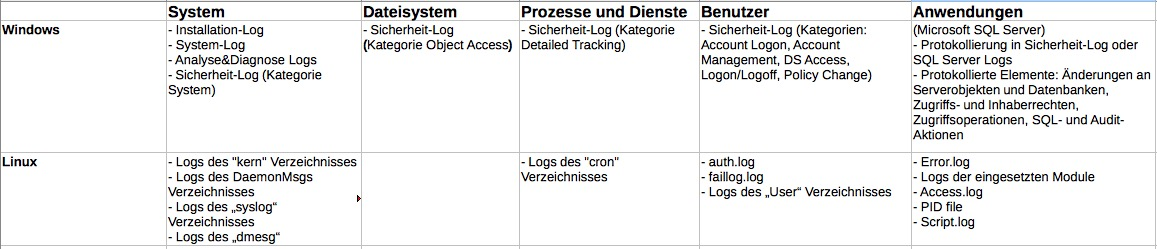
\includegraphics[width=125mm]{Zeichnungen/UnternehmenssystemeInformationen.jpg}
\caption{Placeholder: Darstellung der verfügbaren Informationen der Systeme}
\label{fig:EnterpriseSystemInformation}
\end{figure}

\subsubsection{Netzwerkprotokolle} 
Bzgl. der Netzwerkprotokolle ergeben sich aus der Betrachtung zwei grundlegende Kategorien: \\

Aus den Informationen, die aus den Header-Daten abgeleitet werden können, bildet sich die erste Kategorie. Dies betrifft z.B. die Adressen der Kommunikationspartner, den Nachrichtentyp und anderen Informationen über die Kommunikationsverbindung. Diese Informationen können u.a. verwendet werden, um Hinweise auf die Kommunikation zwischen einem internen System und einem externen Kommunikationspartner nachzuvollziehen oder etwa ungewöhnliche Resourcenanfragen zu erkennen. \\

Die zweite Kategorie bezieht sich auf Informationen, die sich aus dem Mitschnitt einer Kommunikation mithilfe eines Zwischenelementes (z.B. eines Routers, eines Switches, einer Firewall oder einem NIDS) ergeben. Diese Informationen erlauben es, den Ablauf der Kommunikation zu analysieren und das Verhalten der Kommunikationsteilnehmer abzubilden. Sie werden im Folgenden genutzt, um Unregelmäßigkeiten im Protokollablauf, etwa beim Verbindungsaufbau, zu erkennen.

Die folgende Tabelle zeigt die Kategorien im Bezug auf die in diesem Kapitel analysierten Protokolle:
\todoForm{Unternehmensanalyse: Tabelle aktualisieren und in Latex erstellen}

\begin{figure}[h]
\centering
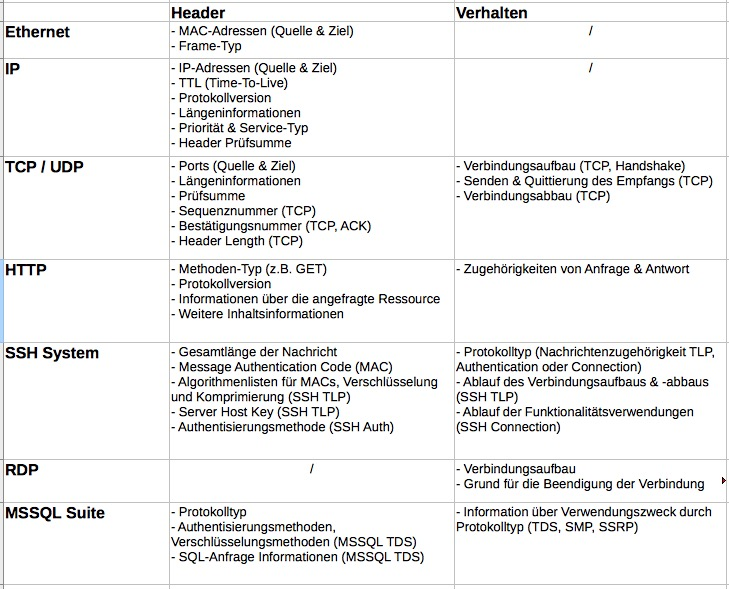
\includegraphics[width=125mm]{Zeichnungen/UnternehmensnetzwerkInformationen.jpg}
\caption{Placeholder: Darstellung der verfügbaren Informationen der Netzwerkprotokolle}
\label{fig:EnterpriseNetworkInformation}
\end{figure}


\subsection{Informationsanalyse am Beispiel einer Malwareinfektion}
Um die Relevanz der dargestellten Kategorien zu verdeutlichen, wird anhand eines Beispieles, die Analyse von Angriffsszenarien bzgl. der Infektion von Systemen durch eine Malware beschrieben. Die Aufgabe eines SIEM-Systems ist es, wie bereits im Grundlagenkapitel beschrieben, Daten über den Status der Systeme im Unternehmensnetzwerk zu sammeln, zu speichern, auszuwerten und zu verknüpfen. Die zu diesem Zweck erstellten und fortlaufend aktualisierten Regeln basieren u.a. auf der Kenntnis des Verhaltens von Malware.

Bei der Infektion, Ausführung und Verbreitung von Malware auf einem System werden Teile des Systems verändert, um eine möglichst lange Ausführung der Malware zu ermöglichen. Diese Veränderungen werden durch das System an verschiedenen Stellen dokumentiert. Diese Daten werden im Rahmen einer Untersuchung und Überwachung eines Systems als Indikatoren für die Kompromittierung eines Systems (IoC, \glqq Indicator of Compromise\grqq ) bezeichnet. Für die Erkennung dieser Indikatoren wird bspw. für die Überwachung der normale Betriebszustand möglichst präzise definiert sowie eine Analyse des infizierten Systems und der darauf befindlichen Malware durchgeführt, durch die potentielle Erkennungsmerkmale festgestellt und zu Indikatoren zusammengestellt werden. Diese werden von einem Sicherheitssystem wie etwa einem Softwareagenten eines SIEM-Systems oder einer Anti-Malware Software für die Erkennung und/oder Schutzmaßnahmen verwendet.

Der Ablauf eines Angriffsszenarios, bei dem eine Malware für einen oder mehrere Zwecke auf einem System installiert wird, lässt sich grob in die folgenden Schritte einteilen:
\begin{enumerate}
\item Erlangen des Zugriffs auf das System über einen Angriffsvektor (z.B. Phishing, infizierte externe Speicher, infizierte Webinhalte)
\item Erstellung eines Zugriffspunktes, Sicherstellung der Persistenz und Verschleierung der Aktivitäten
\item Hinzufügen weiterer Werkzeuge von einem internen oder externen Speicherpunkt
\item Ausführung der Malware auf dem System
\item Ggf. Informationssammlung über weitere Systeme im Netzwerk und Verbreitung der Malware
\end{enumerate}

%Quelle: https://www.fireeye.com/blog/threat-research/2013/12/openioc-series-investigating-indicators-compromise-iocs.html 

Quelle \citep{EntAnalysis1} beschreibt anhand eines Beispieles die Erstellung von IoCs. In diesem Beispiel wird zunächst der Angriffsvektor in Form einer Phishing-E-Mail analysiert. Durch das Herunterladen und den Versuch der Öffnung einer PDF-Datei im Anhang der E-Mail wurde die erste Komponente der Malware platziert, durch die eine Hintertür geöffnet und dem Angreifer Zugriff auf das System verschafft wurde. Bei der Betrachung des Vorfalles durch den zuständigen Analysten konnte dieser Prozess durch dokumentierte Operationen des Betriebssystems nachvollzogen werden. Im Speziellen wurden Operationen im Dateisystem protokolliert, die die Erstellung der PDF-Datei durch Herunterladen des Anhangs (inklusive des dazugehörigen Zeitstempels, Verzeichnispfades und der Betriebssystemoperation) sowie die Erstellung einer Anwendungsdatei (.exe) zum vermuteten Zeitpunkt des Öffnungsversuches durch den Benutzer zeigen. 
Im nächsten Schritt konnten protokollierte Änderungen von Einträgen innerhalb der Windows Registry entdeckt werden sowie weitere Spuren in Form von Dateien und Dateisystemoperationen. Diese zeigten das Hinzufügen weiterer Funktionalität in dem Verzeichnispfad \glqq C:\textbackslash \$RECYCLE.BIN\grqq{} (verstecktes Verzeichnis des Papierkorbes), etwa eines Werkzeuges für die Durchsuchung des Dateisystems,  sowie die Verschleierung der Aktivitäten. Ein typischer Fund konnte etwa das Hinzufügen der Malware in den Autostart-Schlüsseln der Windows Registry verzeichnet werden, durch das die Ausführung der Malware beim Start des Systems sichergestellt werden soll.
Zudem wurde der Aufruf des Verzeichnises per Internet Browser dokumentiert sowie weitere Aktivitäten mit dem Ziel, Informationen über Systeme im lokalen Netzwerk zu sammeln. 

Andere Quellen und Beispiele der Untersuchung von Malware-Typen, u.a. Keylogger-Werkzeugen, Ransomware und trojanischen Pferden ergeben ähnliche Funde \citep{EntAnalysis2}. 
%Quelle: http://hooked-on-mnemonics.blogspot.de/2011/01/intro-to-creating-anti-virus-signatures.html  
Darüber hinaus werden diese Indikatoren auch für die Herstellung von Malware-Signaturen verwendet, die von Anti-Malware-Programmen genutzt werden, um Malware-Infektionen zu erkennen und zu verhindern oder einzudämmen.

Diese Beispiele zeigen, dass die Dokumentation jeglicher Systemprozesse sowie die kontinuierliche Auswertung dieser Dokumentationen essentiell sind, um Angriffe durch Malware-Infektionen zu verhindern. Daraus ergibt sich die Relevanz der Informationsmenge für den Einsatz eines SIEM-Systems.